% !TEX root = ./paper.tex
% Background and motivation

%TODO
%Gives an overview of \tls / \tcp and how they interact. We also need a comparison
%of QUIC and \tls/\tcp on several points that would serve as a base to explain why
%\tls 1.3's extensibility cannot compete with QUIC.
%Gives an overview of \tls / \tcp and how they interact.

%\begin{figure}[!t]
%  \begin{center}
%    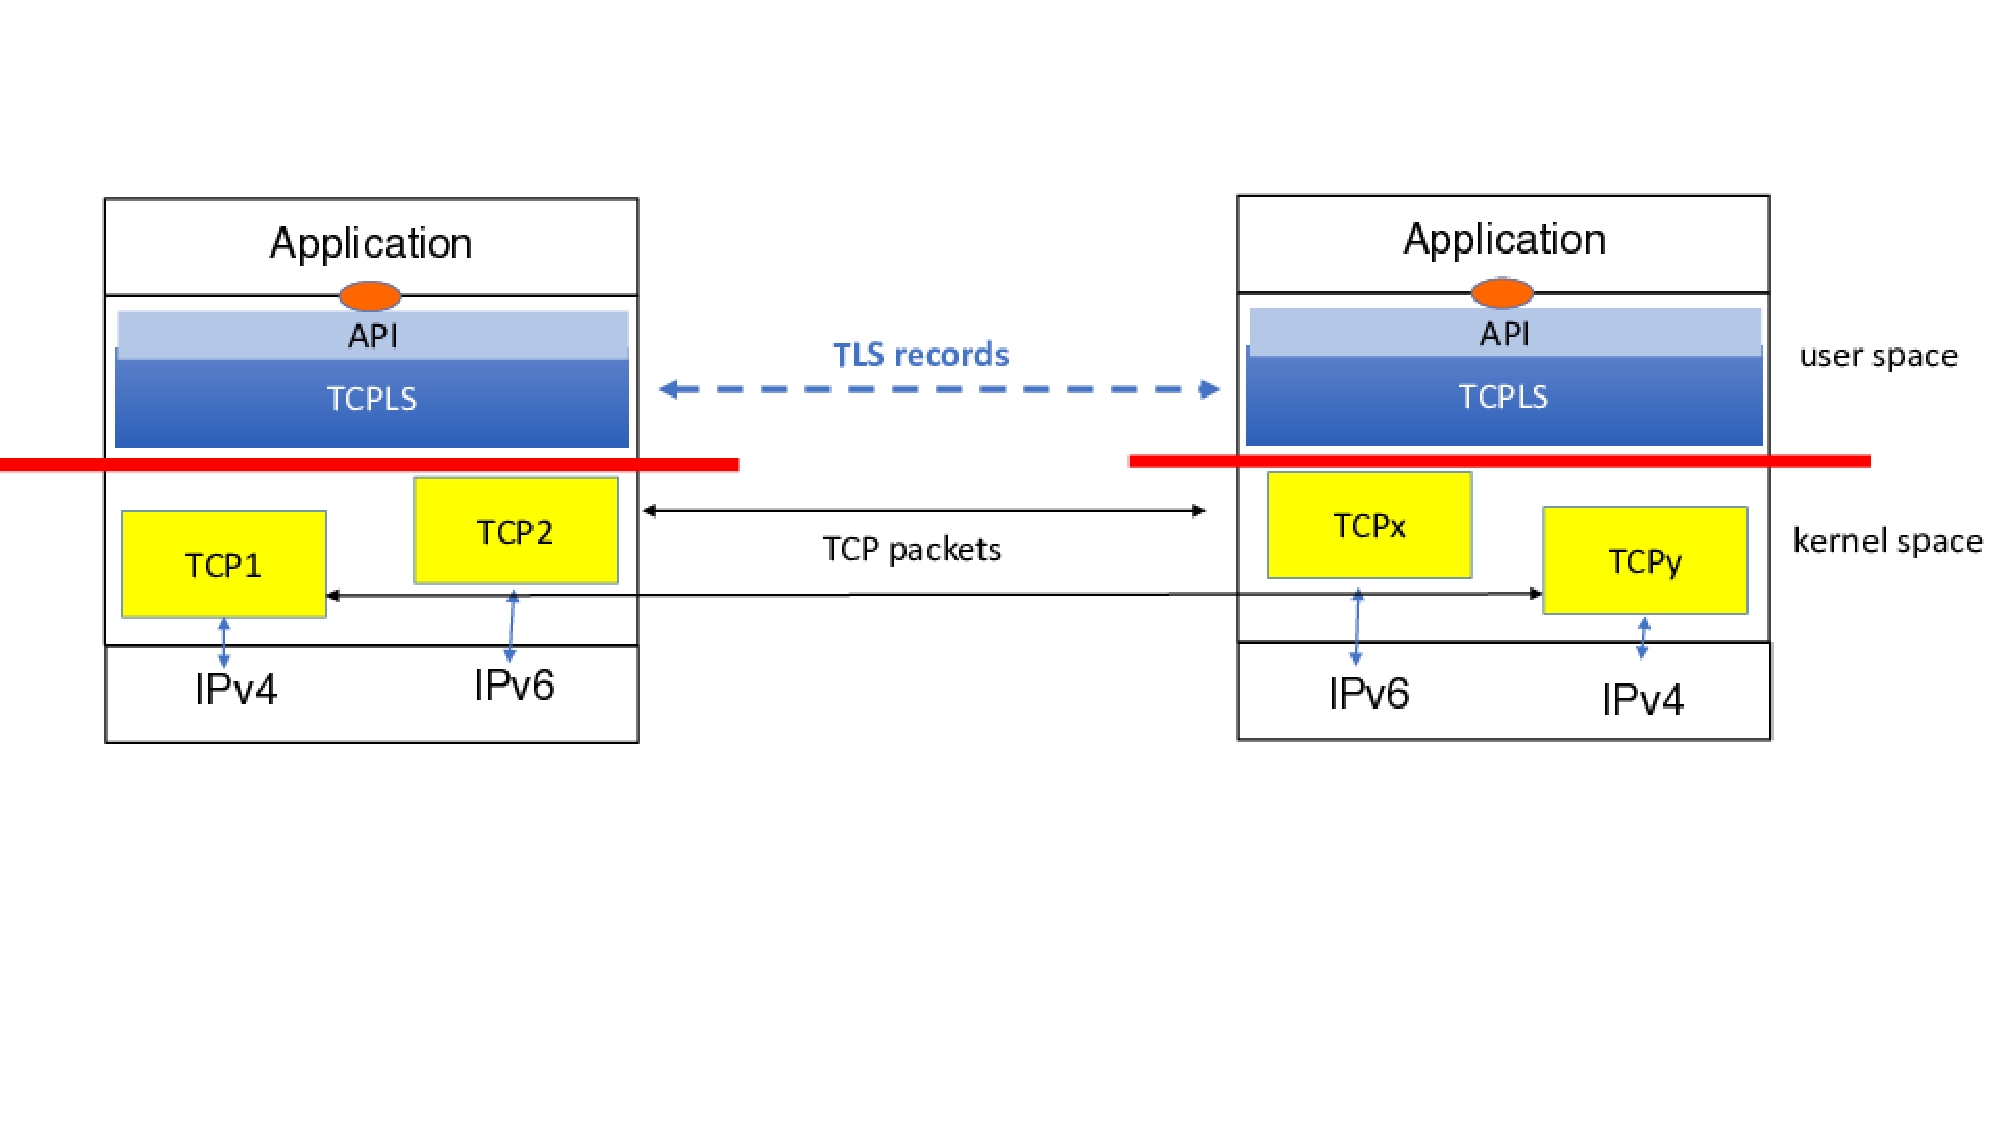
\includegraphics[width=8cm]{figures/tcpls-fig2.pdf}
%  \end{center}
%  \caption{\tcpls in the stack.}
%  \label{fig:arch}
%\end{figure}

 \begin{figure}[!t]
  \begin{center}
\begin{tikzpicture}[node distance=0 cm,outer sep = 0pt,inner sep = 2pt,  scale=0.80, transform shape]
        \tikzset{application/.style={align=center,minimum height=0.3cm,minimum width=10mm}}
        \tikzset{tcpls/.style={align=center,shape=rectangle,fill=green!70!red!100,minimum height=1.5cm,minimum width=22mm,rounded corners, draw}}
         \tikzset{conman/.style={align=center,shape=rectangle,fill=blue!70!green!10,minimum height=0.15cm,minimum width=10mm,rounded corners, draw}}
        \tikzset{api/.style={align=center,shape=rectangle,fill=purple!30,minimum height=0.15cm,minimum width=22mm,rounded corners,draw}}
        \tikzset{tcp/.style={align=center,shape=rectangle,fill=yellow, minimum height=0.4cm,minimum width=5mm,rounded corners,draw}}
        \tikzset{label/.style={align=center,minimum height=0.5cm,minimum width=5mm}}
        \draw(-3,-0.3) rectangle (-0.5,0.4);
        \draw(-3,-3.8) rectangle (-0.5,0.4);
        \draw [red, ultra thick] (-3,-2.5) -- (-0.5,-2.5);
        \draw(-3,-4.5) rectangle (-0.5,-3.8);
        \draw[fill=red!50] (-1.75,-0.3) ellipse (9pt and 4pt);
        \node[application, xshift=-18mm](application){Application};
        \node[tcpls, below= 6.3mm and 0mm of application, xshift=0.3mm](tcpls1){\tcpls};
        \node[api, name=API, below= 3.0mm and 0mm of application, yshift=0mm, xshift=0.3mm ](api1){API};
        \node[conman, name=CM, below= 17mm and 0mm of application](cm1){CM};
        \node[conman, name=CM, below= 7.5mm and 0mm of application](crypto){Crypto};
        \node[tcp, below= 4.5mm and 0mm of tcpls1, xshift=-6mm](tcpx1){\texttt{TCP}$_1$};
        \node[tcp, right=5mm and 0mm of tcpx1, yshift=-4mm, xshift=2mm](tcpy1){\texttt{TCP}$_2$};
        \node[label,  below=8mm and 0mm of tcpx1](ip11){IPV4};
        \node[label,  below=4mm and 0mm of tcpy1](ip12){IPV6};


        \draw(2.3,-0.3) rectangle (4.8,0.4);
        \draw(2.3,-3.8) rectangle (4.8,0.4);
        \draw [red, ultra thick] (2.3,-2.5) -- (4.8,-2.5);
        \draw(2.3,-4.5) rectangle (4.8,-3.8);
        \draw[fill=red!50] (3.6,-0.3) ellipse (9pt and 4pt);
        \node[application, right= 0mm and 43mm of application, xshift=-8mm](application2){ Application};
        \node[tcpls, name=TCPLS, below= 6.3mm and 0mm of application2, xshift=0.3mm](tcpls2){\tcpls};
        \node[api, name=API, below= 3.0mm and 0mm of application2, , xshift=0.3mm](api2){API};
        \node[conman, name=CM, below= 17mm and 0mm of application2](cm2){CM};
        \node[conman, name=CM, below= 7.5mm and 0mm of application2](crypto){Crypto};
        \node[tcp, below= 4.5mm and 0mm of tcpls2, xshift=6mm](tcpx2){\texttt{TCP}$_x$};
        \node[tcp, left=5mm and 0mm of tcpx2, yshift=-4mm, xshift=-0.3mm](tcpy2){\texttt{TCP}$_y$};
        \node[label,  below=8.5mm and 0mm of tcpx2](ip21){IPV4};
        \node[label,  below=4mm and 0mm of tcpy2](ip22){IPV6};

        \node[label,  below=8mm and 0mm of application2, xshift=15mm,rotate=90 ](user1){user space};
        \node[label,  below=33mm and 0mm of application2, xshift=15mm, rotate=90 ](user1){kernel space};

        \node[label,  left=of api2, xshift=-5mm, yshift=-5mm, green!70!red!100 ](user1){\tls records};
        \node[label,  left=of ip22, xshift=-5mm, yshift=10.6mm ](user1){\tcp segments};

        \draw[<->,dotted,green!70!red!100,ultra thick] (tcpls1.east) -- node (line) {} (tcpls2.west);
        \draw[<->,dotted, ultra thick] (tcpx1.east) -- node (line) {} (tcpx2.west);
        \draw[<->,dotted, ultra thick] (tcpy1.east) -- node (line) {} (tcpy2.west);
        \draw[<->, ultra thick] (tcpx1.south) -- node (line) {}(ip11.north);
        \draw[<->, ultra thick] (tcpy1.south) -- node (line) {}(ip12.north);
        \draw[<->, ultra thick] (tcpx2.south) -- node (line) {}(ip21.north);
        \draw[<->, ultra thick] (tcpy2.south) -- node (line) {}(ip22.north);
        \draw[<->,   thick] (cm1.south) -- node (line) {}(tcpx1.north);
        \draw[<->,   thick] (cm1.south) -- node (line) {}(tcpy1.north);
        \draw[<->,   thick] (cm2.south) -- node (line) {}(tcpx2.north);
        \draw[<->,   thick] (cm2.south) -- node (line) {}(tcpy2.north);
\end{tikzpicture}
\end{center}
\vspace{-0.5cm}
\caption{\tcpls is implemented as a user space library. The application controls the streams and the underlying \tcp connections through the API. The crypto module manages the security context and the Connetion Manager (CM) controls the utilization of one or more \tcp connections using the kernel stack.}
 \label{fig:arch}
\end{figure}

\subsection{Overview}
%%%%%%%%%%%%%%%%%%%%%%
Today's applications expect more than a simple bytestream from the transport layer. Security is not anymore a requirement for niche application. Applications expect secure transport by default. Similarly, applications are not restricted anymore on using only one network interface. They need to efficiently deal with IPv6 and IPv4 on dual stack hosts and manage the utilization of different network interfaces on mobile devices such as smartphones. \tcpls provides a fast, flexible, and secure transport protocol that is suited for these modern applications. \tcpls is more than the simple addition of the security features of \tls and the reliability features of \tcp. \tcpls leverages \tls 1.3 to negotiate a security context and uses it to send the user data authenticated and encrypted as \tls records. It leverages these records to establish a secure control channel between the client and server. This channel is used to manage the \tcpls session and exchange all control information without any possible middlebox interference. Finally, \tcpls includes a Connection Manager that controls the underlying \tcp connection. The TLS records of a \tcpls session can be transported over different \tcp connections during the session lifetime. This brings several interesting failover and multipath capabilities. Fig.~\ref{fig:arch} illustrates the interactions between two \tcpls hosts. \tcpls can be implemented in userspace within a library like current \tls implementations. It interacts with the \tcp stack that in our prototype resides in the kernel. The crypto module negotiates and manages the security context while the connection manager (CM) manages the utilization of the underlying \tcp connection(s). Closely coupling \tcp and \tls in \tcpls brings opportunities for performance improvement (e.g., avoiding records fragmentation with dynamic receive buffer auto-tuning and/or with dynamic control of the record length), and for connection reliability (e.g., failover).

%\tcpls (illustrated in Fig.~\ref{fig:arch}) offers a cross-layer interface to \tls and \tcp with the motivation to do more than securing the transport layer. Merging the stacks benefits both protocols and the application using this new approach.
%First, \tcp suffers from a lack of extensibility due to size restrictions in its header and due to potential middlebox interferences~\cite{honda2011still}. \tcpls aims to solve \tcp extensibility issue in the long run by offering a secure control channel to exchange \tcp options without suffering from middlebox interferences and size restrictions in \tcp headers.



%\subsection{Overview}

\tcp separates control information and data by placing the control information
in the packet header and the data in the payload. This separation worked well
until middleboxes started to interfere with \tcp~\cite{10.1145/1064413.1064418,
honda2011still}. On a fraction of Internet paths, including e.g., some enterprise and cellular networks, some middleboxes interfere by adding, removing, or changing \tcp options~\cite{wang2011untold,honda2011still,xu2015investigating} and, in some cases, also transparently terminating \tcp connections. These middleboxes have slowed down the evolution of \tcp in recent years. \tcpls also uses the packet header to exchange \tcp control information, but it leverages the extensibility of \tls 1.3 to place control information including some \tcp options inside the \tls handshake messages and new \tls records. Since this information is encrypted and authenticated, the communicating hosts can exchange new control information without encountering middlebox interference. We refer to this exchange of control information as the secure channel between the two hosts.
%We describe several examples of these new types of
%control information in Sec.~\ref{sec:extending} and Sec.~\ref{sec:connmigr}.

A \tcpls session starts with a secure \tls 1.3 handshake ~\cite{rfc8446}. The
client adds a new \tcpls transport parameter in its \textsc{ClientHello} message. A \tcpls server replies with a \textsc{ServerHello} message that negotiates the security keys and may include additional \tcpls information as
\textsc{EncryptedExtensions}. After this secure handshake, the client and the
server have a shared security context.

As \sctp~\cite{rfc4960} or \quic~\cite{draft-ietf-quic-transport}, \tcpls
supports one or more streams over a single \tcpls session. An application
can open, attach, and close streams to an existing \tcpls session. Each
stream is an independent cryptographic context derived from the \tcpls
security context. The \tcpls streams can carry application data
or control information.

%They must be attached to a \textit{Connected} \tcp bytestream exported as a \texttt{transportid} to the application. To manipulate streams, \tcpls offers an API to open, attach
%and close streams to any available \texttt{transportid} in the \textit{Connected} state, while offering the Stream as the only bytestream abstraction to the upper layer. Streams can only be attached to one \texttt{transportid}, but they can be moved, several streams can be attached to a given \texttt{transportid}, and multiple streams can be attached to multiple \texttt{transportid}s.

To attach a new stream, a host simply sends the \texttt{STREAM\_ATTACH} message as a special \tls record over the secure channel. Since each stream is an independent cryptographic context, the recipient can immediately start to decrypt and extract data from the new stream. No round-trip is wasted to attach a new stream.

%\tcpls can attach streams using the Secure Control Channel and send TLS records
%within them in a zero-rtt fashion. That is, when the peer receives a
%\texttt{STREAM\_ATTACH} message in the control channel, it has everything needed
%to securly derive the right cryptographic context to process the TLS record
%encryted within this stream. No round-trips are needed to attach a new stream.
%Most of records encrypted with a Stream's context contain application data
%transmitted by the client or the server. However, streams can also carry control
%records.

%The control channel between the client and the server
%enables \tcpls to define a new bytestream abstraction and support many new
%features while benefitting from the current kernel and network optimization for
%\tcp performance.

%Applications such as HTTP/2 support multiple streams mapped to a single \tcp
%connection. However, there are situations, e.g., to prevent head-of-line
%blocking, where different streams should be mapped over other underlying \tcp
%connections. With \tcpls, the client and the server can establish different
%datastreams over a single \tcpls session, preventing \tcp's HOL. Thus, a
%\tcpls session can be composed of one or more \tcp connections similarly as a
%\mptcp connection gathers subflows.

\tcpls' Connection Manager controls the utilization of the underlying \tcp connections. It can open, close, or reestablish failed \tcp connections. Each of
the connections that composes a \tcpls session is identified by a \emph{transport identifier}. By default, the data from a stream can be sent over any of the underlying \tcp connections. The applications that require finer control over the utilization of the underlying \tcp connections can use the \tcpls API to map a stream on a specific underlying connection. In this case, all the data of this stream is exchanged over this specific connection. By placing two streams on different connections, an application can prevent Head-Of-Line (HOL) blocking among these streams.

\tcpls also supports failover and multipath. To support these features, it
must be possible to send data from a given stream over different \tcp connections. In this case, the \tcp level sequence numbers and acknowledgements are not sufficient anymore to enable the receiver to reorder the data. When this feature
is enabled, \tcpls its own sequence numbers and acknowledgements that are exchanged as new \tls records over the secure control channel.
Thanks to these \tcpls acknowledegments, a \tcpls session can survive to
the failure of the underlying \tcp connection by reestablishing a new
\tcp connection to continue the data transfer and replay the lost records.

A \tcp connection ends with the exchange of \fin or \rst packets. However, some
middleboxes force the termination of \tcp connections by sending \rst
packets~\cite{rfc3360,weaver2009detecting}. \tcpls can preserve established
connections by automatically restarting the underlying \tcp connection upon
reception of a spurious reset. \tcpls defines the connection termination at the
stream level: a \tcpls session is closed once the last stream attached to a
\tcp connection is securely closed.

That is, \tcpls' Secure Control Channel provides a flexible abstraction
to the upper layer that supports various new features such as
Streams, connection reliability, different secure multipath modes, secure
connection closing, encrypted \tcp options and leverages \tcp's performance and \tls's state of deployment.

%Todo explain that the transport abstraction level failed to offera versatile
%usage
%of the transport layer, and explain how a session layer can repair the
%abstraction
%Besides, with our design of \tcp extensibility
%within \texttt{\tcpLS}, applications would be able to tune \tcp on a connection basis,
%using existing options or any future option without middlebox interferences. As
%a matter of example, our \texttt{\tcpLS} implementation supports several
%\tcp options that can difficulty live at the \tcp layer
%(e.g., Joining a Multipath connection, injecting eBPF bytecode to the kernel's
%peer to tune \tcp). With \texttt{TCPLS}, we show how to solve several of these
%existing problem.

%Finally, \texttt{\tcpLS}'s control channel is expected to offer extensibility
%without middlebox interference and with protocol message indistinguishability
%from the network to avoid fingerprinting of the client stack. Our objective is
%to design a versatile \tcp extensibility mechanism that would allow to set
%options, exchange eBPF bytecode~\cite{de2019pluginizing} to tune the peer's kernel and implement new
%session behaviours.
